\documentclass[a4paper, 12pt]{scrartcl}

\usepackage[utf8]{inputenc}
\usepackage[T1]{fontenc}
\usepackage[ngerman]{babel}

\usepackage{amssymb}
\usepackage{amsmath}

\usepackage{eurosym}
\usepackage{framed}

\usepackage[hidelinks]{hyperref}
\usepackage{float}

\usepackage{tikz}
\usetikzlibrary{arrows, arrows.meta, patterns}

\tikzstyle{arrow}=[-{Latex[length=3mm, width=1.8mm]}]

\allowdisplaybreaks
\newcommand{\tagyoureit}{\addtocounter{equation}{1}\tag{\theequation}}
\renewcommand{\labelenumi}{(\arabic{enumi})}
\renewcommand{\labelenumii}{(\alph{enumii})}

\setlength{\parindent}{0pt}

\title{Aufgabe 2\\Wehret den Wildschweinen!\\Dokumentation}
\author{Kamal Abdellatif}
\date{}

\begin{document}
\maketitle

\section{Kritischer Pfad}
Das Ziel der Erdarbeiten ist es, dass jeder Weg für ein Wildschwein vom Nordrand zum Südrand mindestens einmal einen Höhenunterschied von mehr als einem Meter beinhaltet. Der \emph{Weg} eines Wildschweins sei dabei die Abfolge von besuchten Planquadraten. Geht ein Wildschwein von einem Planquadrat zu einem benachbarten Planquadrat, überschreitet es dabei die \emph{Grenze} zwischen beiden Quadraten. Kann eine Grenze von einem Wildschwein nicht mehr bewältigt werden, da der Betrag der Höhendifferenz größer gleich einem Meter ist, handelt es sich um eine \emph{kritische} Grenze.

Das Ziel ist genau dann erfüllt, wenn mindestens ein zusammenhängender Pfad aus kritischen Grenzen vom Linken zum rechten Feldrand besteht. Ein solcher Pfad ist ein \emph{kritischer} Pfad. Existiert kein kritischer Pfad, so gibt es immer einen Weg für ein Wildschwein, der durchgehend passierbar ist.
\begin{figure}[H]
	\centering\sffamily\Large
	\begin{tikzpicture}[scale=.85]
		\draw[very thick] (0, 0) rectangle (12, 6);
		\draw[ultra thick] (0, 2) to (1, 2) to (1, 1) to (4, 1) to (4, 3) to (2, 3) to (2, 5) to (7, 5) to (7, 3) to (9, 3) to (9, 2) to (12, 2);
		\path[arrow, shorten >=2mm, dashed, thick]
			(2.5, 6) edge +(0, -1)
			(3.5, 6) edge +(0, -1)
			(3.5, 6) edge +(0, -1)
			(4.5, 6) edge +(0, -1)
			(5.5, 6) edge +(0, -1)
			(6.5, 6) edge +(0, -1)
			(0.5, 6) edge +(0, -4)
			  (8, 6) edge[bend left=10] +(-.8, -3)
			(8.5, 6) edge +(0, -3)
			(9.5, 6) edge +(0, -4)
			(10.5, 6) edge +(0, -4)
			(11, 6) edge[bend right=10] (11.8, 2);
		\draw[dashed, thick] (1.5, 6) edge +(0, -3.5);
		\path[arrow, shorten >=2mm, dashed, thick] (1.5, 3)
			edge[out=-90, in=90] (1.5, 1)
			edge[out=-90, in=170] (4, 1.3)
			edge[out=-90, in=190] (4, 2.5);
		\node[above] at (6, 6) {N};
		\node[right] at (12, 3) {O};
		\node[below] at (6, 0) {S};
		\node[left] at (0, 3) {W};
		\end{tikzpicture}
	\caption{Kritischer Pfad}
\end{figure}
Das Problem wird gelöst, indem ein kritischer Pfad mit minimalen Erdarbeiten konstruiert wird. Da beide Problemstellungen äquivalent sind, entspricht die minimale Lösung des kritischer Pfads der Lösung des ursprünglichen Problems.

Ist ein gewählter Pfad noch nicht kritisch, so sind von Wildschweinen noch passierbare Grenzen enthalten. Um eine Lösung zu finden werden diese Grenzen durch Erdarbeiten in kritische Grenzen umgewandelt.
\subsection{Umbau von Grenzen}
Es seien zwei benachbarte Planquadrate der Höhen $a$ und $b$, deren gemeinsame Grenze nach Bearbeitung kritisch sein soll. Die zu erfüllende Bedingung lautet, dass der Betrag der Höhendifferenz $\Delta = |a-b|$ größer gleich 1 ist.\footnote{Die Einheiten Meter und Euro werden gleich 1 gesetzt. Es gilt $1 \mathrm{m} = 100\text{\euro} = 1$} Es sollen dabei nur Erdarbeiten bezüglich den beiden betrachteten Planquadrate unternommen werden. Um die Differenz zu erhöhen, ist es immer günstiger, den schon bestehenden Höhenunterschied zu vergrößern.
\begin{figure}[H]
	\centering
	\begin{tikzpicture}
		\clip (-1, 0) rectangle (6, 5);
		\draw[very thick] (0, 0) -- ++(0, 2) -- node[below=5mm] {$a$} ++(2, 0) -- (2, 0) -- ++(0, 3) -- node[below=5mm] {$b$} ++(2, 0) -- (4, 0);
		\draw[|-|] (-.5, 2) -- node[right] {$\Delta$} +(0, 1);
	\end{tikzpicture}
	\begin{tikzpicture}
		\clip (-1, 0) rectangle (6, 5);
		\draw[very thick, dashed] (0, 0) -- ++(0, 2) -- ++(2, 0) -- (2, 0) -- ++(0, 3) -- ++(2, 0) -- (4, 0);
		\draw[very thick] (0, 0) -- ++(0, 1) -- node[below=5mm] {$a'$} ++(2, 0) -- (2, 0) -- ++(0, 4) -- node[above=5mm] {$b'$} ++(2, 0) -- (4, 0);
		\draw[-{angle 60}, line width=1mm] (1, 1.5) to[out=90, in=110, looseness=2] (3, 3.5);
		\draw[|-|] (4.5, 1) -- node[right] {$\Delta' \ge 1$} +(0, 3);
		\node at (1.2, 4) {$w$};
	\end{tikzpicture}
	\caption{Umschaufeln zur kritischen Kante}
\end{figure}
Dazu wird Erde vom niedrigeren Quadrat $a$ (o.\,B.\,d.\,A) zum höheren Quadrat $b$ geschaufelt. Wurden $w$ Erdarbeiten auf diese Weise verrichtet, gilt für die jeweiligen Höhen $a'$ und $b'$ nach verrichteter Arbeit
\begin{equation*}
	a' = a - w \qquad b' = b + w
\end{equation*}
Um die genannte Bedingung zu erfüllen, muss für die neue Differenz $\Delta'$ gelten
\begin{align*}
	 1&\le \Delta'  \\
	 &\le b' - a' \tag{$b' > a'$}\\
	 &\le (b+w) - (a - w)\\
	 2w &\le 1 - (b-a)\\
	 w &\le \frac{1}{2}(1 - \Delta) \tagyoureit\label{eq:arbeit}
\end{align*}
\begin{figure}[H]
	\centering
	\begin{tikzpicture}
		\draw[-{Latex[length=3mm]}] (0, -1) to (0, 2.5) node[above] {$w$};
		\draw[-{Latex[length=3mm]}] (-5, 0) to (5, 0) node[right] {$(a-b)$};
		\draw (-2, .1) to +(0, -.2) node[below] {$-1$};
		\draw  (2, .1) to +(0, -.2) node[below] {$1$};
		\draw[very thick, shorten >=2mm] (-5, 0) -- (-2, 0) -- (0, 1.5) -- (2, 0) -- (5, 0);
		\draw[dashed, thick] (-4, 1.5) -- (4, 1.5) node[right] {$\displaystyle w_{max}=\frac{1}{2}$};
	\end{tikzpicture}
	\caption{Benötigte Erdarbeiten $w$ in Abh. von der Höhendifferenz}
\end{figure}
Aus letzerer Gleichung folgt die minimale Menge an Erdarbeiten zum Umbauen einer Grenze mit Höhenunterschied $\Delta$ zu einer kritischen Grenze.
\subsection{Pfad-Heuristik}
\label{subsec:heuristik}
Zur Minimierung der Kosten wird der Pfad gewählt, der am wenigsten Gesamt-Erdarbeiten erfordert um kritisch zu werden. Es bietet sich an, die gesamten Erdarbeiten als Summe der einzeln benötigten Arbeiten aller Grenzen nach Gleichung \eqref{eq:arbeit} zu errechnen. Allerdings gilt dies nur unter der Annahme, dass einzelne Erdarbeiten an verschiedenen Grenzen unabhängig voneinander sind. Leider ist dies nicht der Fall. Liegen zwei Grenzen am selben Planquadrat an, tritt einer von zwei Fällen auf:
\begin{enumerate}
	\item Die jeweiligen Erdarbeiten der Grenzen entnehmen beide dem Planquadrat Erde oder fügen ihm beide Erde hinzu.
	\item Eine Grenze entnimmt Erde, während die andere Erde hinzufügt.
\end{enumerate}
Im ersten Fall wird überflüssige Arbeit verrichtet: Nach dem ersten Umschaufeln liegt das Quadrat bereits weiter in der erwünschten Richtung der zweiten Grenze, sodass weniger Erde umgeschaufelt werden muss. Im zweiten Fall kommt es zu einem Interessenkonflikt, durch welchen nach Tätigung beider Arbeiten nicht garantiert werden kann, dass nun beide kritisch sind. Es muss mehr Erdarbeit verrichtet werden, da geschaufelte Erde für eine Grenze mehr Arbeit für die Andere bedeutet.

\begin{minipage}[t]{.45\textwidth}
	\begin{figure}[H]
		\centering
		\begin{tikzpicture}
			\clip (0, .2) rectangle (6, 4.7);
			\draw[very thick]
				(0, 0) rectangle (2, 1)
				(2, 0) rectangle (4, 3)
				(4, 0) rectangle (6, 2);
			\draw[white, very thick] (0, 0) -- (6, 0);
			\draw[-{angle 60}, shorten >=2mm, line width=1mm] (1, .75) to[out=90, in=110, looseness=1.8] (2.8, 3.5);
			\draw[-{angle 60}, shorten >=2mm, line width=1mm] (5, 1.75) to[out=90, in=80, looseness=1.8] (3.2, 3.5);
			\draw[very thick, dashed] (0, .5) -- +(2, 0) (4, 1.5) -- +(2, 0) (2, 3) rectangle +(2, 1);
		\end{tikzpicture}
		\caption{Fall (1)}\label{fig:fall1}
	\end{figure}
\end{minipage}\hfill
\begin{minipage}[t]{.45\textwidth}
	\begin{figure}[H]
		\centering
		\begin{tikzpicture}
			\clip (0, .2) rectangle (6, 4.7);
			\draw[very thick]
				(0, 0) rectangle (2, 1)
				(2, 0) rectangle (4, 1.7)
				(4, 0) rectangle (6, 3);
			\draw[white, very thick] (0, 0) -- (6, 0);
			\draw[-{angle 60}, shorten >=2mm, line width=1mm] (1, .75) to[out=90, in=110, looseness=1.8] (2.8, 2.5);
			\draw[-{angle 60}, shorten <=2mm, line width=1mm] (3.2, 2.5) to[out=90, in=110, looseness=1.8] (5, 3.25);
			\draw[very thick, dashed] (0, .5) -- +(2, 0) (4, 3) rectangle +(2, .5);
			\fill[pattern=north east lines] (2, 1.7) rectangle +(2, .8);
			\draw[dashed, very thick] (2, 1.7) rectangle +(2, .8);
			\node[fill=white, inner sep=1mm] at (3, 2.1) {\bfseries\large!};
		\end{tikzpicture}
		\caption{Fall (2)}\label{fig:fall2}
	\end{figure}
\end{minipage}
Die Summe der einzelnen Erdarbeiten kann nicht als exaktes Maß für die benötigten Erdarbeiten zur Umsetzung eines Pfades gewählt werden. Stattdessen wird diese Größe als Heuristik verwendet werden, um verschiedene Pfade gegeneinander abzuwägen.
\begin{framed}
	Die Heuristik wählt den Pfad von Westrand zu Ostrand, welcher die geringste Summe an Erdarbeiten für die einzelnen Grenzen aufweist. Dieser Pfad ist der \emph{minimale} Pfad.
\end{framed}
Dies erzeugt nicht notwendigerweise die optimale Lösung, läuft aber dafür in akzeptabler Laufzeit. Genaueres zur optimalen Lösung siehe Sektion (?).%TODO DO ME

Das Problem des minimalen Pfads wird in einen Graphen $G(V,\ E)$ eingebettet. Jede Kante stellt eine Grenze auf dem Brachland dar. Die Knoten liegen auf den Eckpunkten der Planquadrate. Da die Ränder abgezäunt sind, werden Grenzen vernachlässigt, die direkt am West- oder Ostrand anliegen. Der Nord- und Südrand des Brachlandes wird für die Wildschweine immer als passierbar angenommen: Jedes Wildschwein startet auf einem Planquadrat am Nordrand und läuft zu einem Planquadrat am Südrand. Somit fallen auch Grenzen weg, welche inzident zu mindestens einem Knoten am Rand sind.\\

Die Gewichtung $w(e)$ für jede Kante $e \in E$ entspricht den nach Gleichung (\ref{eq:arbeit}) benötigten Erdarbeiten zum Umbau zu einer kritischen Grenze. Die \emph{Länge} eines Pfads innerhalb des Graphen $G$ entspricht demnach der Summe der Einzel-Erdarbeiten. Der minimalen Pfad von Westrand zum Ostrand ist der kürzeste Pfad von einem Knoten am Westrand zu einem Knoten am Ostrand im Graphen.

Es werden zwei virtuelle Knoten $s$ und $t$ mit einer Kante an alle Knoten des Westrandes beziehungweise des Ostrandes angefügt. Die Gewichtung dieser Kanten sei 0. Auf diese Weise wurde das Problem auf den kürzesten Pfad vom Knoten $s$ zu Knoten $t$ reduziert.
\begin{figure}[H]
	\centering
	\begin{tikzpicture}[scale=.78, thick]
		\draw[line width=1mm, opacity=.2] (-1, -1) rectangle (6, 5);
		\node[above] at (2.5, 5) {\sffamily N};
		\node[below] at (2.5, -1) {\sffamily S};
		\node[draw, circle, inner sep=3pt] (s) at (-4, 2) {$s$};
		\node[draw, circle, inner sep=3pt] (t) at (9, 2) {$t$};
		\foreach \x in {0,...,5}{
			\draw (\x, 0) -- (\x, 4);
			% \draw[line width=1mm, opacity=.2] (\x, -1) -- (\x, 5);  % Grid lines
		}
		\foreach \y in {0,...,4}{
			\draw[dashed] (s) -- (-1, \y) (6, \y) -- (t);
			\draw (-1, \y) -- (6, \y);
			% \draw[line width=1mm, opacity=.2] (-1, \y) -- (6, \y);
		}
		\foreach \x in {-1,...,6}{
			\foreach \y in {0,...,4}{
				\draw[fill=white] (\x, \y) circle (2mm);
			}
		}
	\end{tikzpicture}
	\caption{Einbettung in einen Graphen}
\end{figure}
Um den kürzesten Pfad zu erhalten, wird \textsc{Dijkstra}'s Algorithmus\cite{dijkstra} für den kürzesten Pfad im ungerichteten kanten-gewichteten Graphen auf $G$ angewendet. Die minimalen Pfade zu den vorgegebenen Beispielen sind im Anhang \eqref{app:paths} beigefügt.
\section{Dualgraph}
Ist durch die Heuristik ein minimaler Pfad ermittelt worden, gilt es diesen umzubauen, sodass ein kritischer Pfad entsteht. Die dazu unternommenen Erdarbeiten sollen dabei folgende Ziele verfolgen: (siehe Sektion \ref{subsec:heuristik})
\begin{enumerate}
	\item Ausnutzen von begünstigenden Umständen
	\item Lösen von eventuellen Konflikten
\end{enumerate}
Um die genannten Fälle zu erkennen und umzusetzen, wird ein Dualgraph erzeugt. In diesem Graphen werden die Relationen zwischen voneinander abhängigen Erdarbeiten dargestellt, welche von der Heuristik bisher vernachlässigt wurden.

Alle Erdarbeiten sollen zur Vereinfachung nur über Grenzen des gewählten Pfades getätigt werden. Demnach finden Veränderungen nur in den am Pfad direkt anliegenden Planquadraten statt.\footnote{Der Einbezug außen liegender Quadrate erweist sich in Sonderfällen zwar als günstiger, bedeutet aber unverhältnismäßig mehr Komplexität in die Lösung des Problems. Mehr zu Sonderfällen in Sektion (?)} % TODO

Alle am Pfad anliegenden Planquadrate sind in einem Knoten im Dualgraphen repräsentiert. Liegt die Grenze zwischen zwei benachbarten Quadraten auf dem Pfad, so wird eine gerichtete Kante zwischen den jeweiligen Knoten im Dualgraph gezogen. Die Richtung der Kante zeigt dabei immer vom niedrigeren Quadrat zum höheren Quadrat. 
\begin{figure}[H]
	\centering
	\begin{tikzpicture}[scale=1.5, thick]
		\foreach \x in {0,...,5}{
			\draw[opacity=.2] (\x, -.25) -- (\x, 4.25);
		}
		\foreach \y in {0,...,4}{
			\draw[opacity=.2] (-.25, \y) -- (5.25, \y);
		}
		\foreach \pos in {(0, 0), (1, 0), (1, 1), (1, 2), (3, 2)}{
			\draw[very thick, -{latex}, shorten >=3mm] \pos++(.5, .5) to ++(0, 1);
		}
		\draw[very thick, {latex}-, shorten <=3mm] (2, 2)++(.5, .5) to ++(0, 1);
		\draw[very thick, {latex}-, shorten <=3mm] (4, 1)++(.5, .5) to ++(0, 1);
		\foreach \pos in {(0, 0), (1, 1), (0, 2), (3, 2)}{
			\draw[very thick, -{latex}, shorten >=3mm] \pos++(.5, .5) to ++(1, 0);
		}
		\draw[line width=1mm] (-.5, 1) to (2, 1) to (2, 2) to (1, 2) to (1, 3) to (4, 3) to (4, 2) to (5.5, 2);
		\foreach \pos in {(0, 0), (0, 1), (1, 0), (1, 1), (2, 1), (0, 2), (1, 2), (2, 2), (3, 2), (4, 2), (4, 1), (1, 3), (2, 3), (3, 3)}{
			\draw[fill=white] \pos++(.5, .5) circle (2mm);
		}
	\end{tikzpicture}
	\caption{Kritischer Pfad mit entsprechendem Dualgraph}
\end{figure}
Der Dualgraph ist meist nicht zusammenhängend. Unverbundene Teile des Graphen haben keinerlei Relation zwischeneinander, sodass sie unabhängig betrachtet werden können.
\begin{figure}[H]
	\centering
	\begin{tikzpicture}[scale=1.5, thick]
		\foreach \pos in {(0, 0), (1, 0), (1, 1), (1, 2), (3, 2)}{
			\draw[very thick, -{latex}, shorten >=3mm] \pos++(.5, .5) to ++(0, 1);
		}
		\draw[very thick, {latex}-, shorten <=3mm] (2, 2)++(.5, .5) to ++(0, 1);
		\draw[very thick, {latex}-, shorten <=3mm] (4, 1)++(.5, .5) to ++(0, 1);
		\foreach \pos in {(1, 1), (0, 2), (3, 2)}{
			\draw[very thick, -{latex}, shorten >=3mm] \pos++(.5, .5) to ++(1, 0);
		}
		\foreach \pos in {(0, 0), (0, 1), (1, 0), (1, 1), (2, 1), (0, 2), (1, 2), (2, 2), (3, 2), (4, 2), (4, 1), (1, 3), (2, 3), (3, 3)}{
			\draw[fill=white] \pos++(.5, .5) circle (2mm);
		}
	\end{tikzpicture}
	\caption{Unabhängige Teilgraphen}
\end{figure}
Es gilt im Folgenden, einen einzelnen zusammenhängenden Teilgraphen von Konflikten zu befreien.
\subsection{Konfliktlösung}
Die naiven Erdarbeiten, von welchen in der Heuristik ausgegangen wurden, sind im Dualgraph wiedererkennbar: Da die Arbeit an einer Grenze immer in Richtung des schon bestehenden Gefälle stattfindet, zeigen die Kanten direkt Richtung der Erdarbeiten, die an jeder Grenze geplant waren. Für Knoten bedeuten eingehende Kanten Zugeschaufelte, ausgehende Kanten abgetragene Erde.

Knoten, welche sowohl eingehende als auch ausgehende Kanten haben, bergen Konflikte. Knoten hingegen, die ausschließlich indizent zu ein- oder ausgehenden Kanten sind, ermöglichen Einsparungen in Erdarbeiten.

\begin{minipage}[t]{.45\textwidth}
	\begin{figure}[H]
		\centering
		\begin{tikzpicture}[very thick]
			\node[draw, circle, minimum width=1cm] (n) at (0, 0) {};
			\path[-{Latex[width=2.5mm, length=4mm]}]
			(-2, 0) edge (n)
			(0, -2) edge (n)
			(0, 2) edge (n)
			(2, 0) edge (n);
		\end{tikzpicture}
		\caption{Konfliktfreier Knoten (Fall 1)}
	\end{figure}
\end{minipage}\hfill
\begin{minipage}[t]{.45\textwidth}
	\begin{figure}[H]
		\centering
		\begin{tikzpicture}[very thick]
			\node[draw, circle, minimum width=1cm] (n) at (0, 0) {};
			\path[-{Latex[width=2.5mm, length=4mm]}]
			(-2, 0) edge (n)
			(n) edge (2, 0)
			(0, 2) edge (n)
			(n) edge (0, -2);
		\end{tikzpicture}
		\caption{Knoten mit konfliktierenden Kanten (Fall 2)}
	\end{figure}
\end{minipage}
\newpage
\paragraph{Eigenschaften eines konfliktfreien Graphs}
Ein vollständig konfliktfreier Graph besteht nur aus Knoten von Fall (1): Jeder Knoten besitzt entweder nur eingehende oder ausgehende Kanten. Die Ausrichtung der Kanten sei dabei die \emph{Ausrichtung} des Knoten. Es können zwei adjazente Knoten nicht beide eingehend oder ausgehend sein, da die geteilte Kante immer entgegengesetzte Ausrichtungen impliziert.
\begin{framed}
	Adjazente Knoten besitzen verschiedene Ausrichtungen.
\end{framed}
Der Graph muss demnach 2-knotenfärbbar sein. Dass dies immer der Fall ist wird in Sektion \eqref{par:faerbung} dargelegt.
\begin{figure}[H]
	\centering
	\begin{tikzpicture}[scale=1.5, thick]
		\foreach \pos in {(0, 0), (2, 2), (1, 1)}{
			\draw[very thick, -{latex}, shorten >=3mm] \pos to ++(0, 1);
		}
		\foreach \pos in {(1, 2), (1, 0), (3, 2), (4, 1)}{
			\draw[very thick, {latex}-, shorten <=3mm] \pos to ++(0, 1);
		}
		\foreach \pos in {(1, 1), (0, 2), (2, 2)}{
			\draw[very thick, -{latex}, shorten >=3mm] \pos to ++(1, 0);
		}
		\foreach \pos in {(0, 1), (1, 2), (3, 2)}{
			\draw[very thick, {latex}-, shorten <=3mm] \pos to ++(1, 0);
		}
		\foreach \pos in {(0, 0), (1, 1), (0, 2), (2, 2), (4, 2), (1, 3), (3, 3)}{
			\draw[fill=blue!20] \pos circle (2mm);
		}
		\foreach \pos in {(0, 1), (1, 0), (2, 1), (1, 2), (3, 2), (4, 1), (2, 3)}{
			\draw[fill=red!20] \pos circle (2mm);
		}
	\end{tikzpicture}
	\caption{2-Färbung eines konfliktfreien Graphs}
\end{figure}
\paragraph{Bearbeitung durch Kantendrehung}
Um einen solchen Zustand ausgehend von einem konfliktierten Graphen zu erreichen müssen Kanten in ihrer Ausrichtung verändert werden. Genauer, kehrt sich die Richtung einer Kante $(a, b)$ um zu der Kante $(b, a)$, so sei diese Kante \emph{gedreht}.

Die Drehung einer Kante erfordert Erdarbeiten. Da danach das Gefälle umgekehrt ist, muss zusätzlich Arbeit verrichtet werden, das vorherige Gefälle auszugleichen, bevor das entgegen gesetzte Gefälle geschaufelt wird. Das Ausgleichen der Differenz $\Delta$ kostet dabei $\frac{1}{2}\Delta$, und das Aufschaufeln der neuen Differenz von 1 kostet $\frac{1}{2}$. Somit gilt für die zusätzliche Erdarbeit $\delta w$
\begin{align*}
	w + \delta w &= \frac{1}{2}\Delta + \frac{1}{2} \\
	\frac{1}{2}(1 - \Delta) + \delta w &= \frac{1}{2}(1 + \Delta) \\
	\delta w &= \Delta \tagyoureit\label{eq:deltaw}
\end{align*}

Es sind immer zwei verschiedene Färbungen möglich, die das jeweilige Komplimentär des Anderen sind. Je nach Färbung werden unterschiedliche Kanten gedreht, welche nach Gleichung \eqref{eq:deltaw} verschiedene Mengen an Erdarbeit hinzufügen. Es wird die Färbung gewählt, die die geringere Summe an zusätzlichen Arbeiten benötigt.
\paragraph{2-Färbung des Graphen}
\label{par:faerbung}
Für die 2-Färbung eines Graphen $G(V,\ E)$ müssen alle Knoten in einer von zwei disjunkten Mengen $S_0,\ S_1 \subseteq V$ enthalten sein, wobei keine zwei adjazenten Knoten in der selben Menge enthalten sind.
\[ (a,\ b) \in E \Rightarrow (a \in S_0 \Leftrightarrow b \in S_1) \qquad (S_0 \cup S_1 = V)\]
Es sei $\mu$ eine Abbildung von der Menge aller Knoten auf zwei diskrete Werte. Der abgebildete Wert eines Knoten $v$ gibt vor, in welcher der beiden Mengen $v$ enthalten ist.
\[ \mu : V \rightarrow \{0,\ 1\} \qquad v \in S_i \Leftrightarrow \mu(V) = i \]
Jeder Knoten $v$ im Dualgraph besitzt Koordinaten $x(v),\ y(v)$ der Position des entsprechenden Planquadrats auf dem Brachland. Es sei
\begin{equation}
	\mu(v) = x(v) + y(v) \mod 2 \label{eq:abbildung}
\end{equation}
Zwei benachbarte Planquadrate unterscheiden sich entweder in $x$- oder $y$-Koordinate um genau 1. Demnach ist die Differenz zwischen der Summe der jeweiligen Koordinaten zweier benachbarter Quadrate immer genau 1. Zwei um 1 verschiedene Zahlen besitzen unterschiedliche Reste für Modulo 2.
\begin{align*}
	(a,\ b) \in E &\Rightarrow \left|\mu(a) - \mu(b)\right| = 1 \\
	\therefore \mu(a) = 0 &\Leftrightarrow \mu(b) = 1
\end{align*}
\begin{flushright}
	\Large$\square$
\end{flushright}

Die Abbildung $\mu$ erzeugt ein Schachbrettmuster, welches über den Dualgraphen gelegt wird. Bei der Verwendung von $\mu$ als Bildungsvorschrift ist eine korrekte Färbung garaniert.
\begin{figure}[H]
	\centering
	\begin{tikzpicture}[scale=1.5, thick]
		\foreach \pos in {(0, 0), (2, 2), (1, 1)}{
			\draw[very thick, -{latex}, shorten >=3mm] \pos to ++(0, 1);
		}
		\foreach \pos in {(1, 2), (1, 0), (3, 2), (4, 1)}{
			\draw[very thick, {latex}-, shorten <=3mm] \pos to ++(0, 1);
		}
		\foreach \pos in {(1, 1), (0, 2), (2, 2)}{
			\draw[very thick, -{latex}, shorten >=3mm] \pos to ++(1, 0);
		}
		\foreach \pos in {(0, 1), (1, 2), (3, 2)}{
			\draw[very thick, {latex}-, shorten <=3mm] \pos to ++(1, 0);
		}
		\foreach \pos in {(0, 0), (1, 1), (0, 2), (2, 2), (4, 2), (1, 3), (3, 3), (0, 1), (1, 0), (2, 1), (1, 2), (3, 2), (4, 1), (2, 3)}{
			\draw[fill=white] \pos circle (2mm);
		}
		\foreach \pos in {(0, 0), (0, 2), (1, 1), (1, 3), (2, 0), (2, 2), (3, 1), (3, 3), (4, 0), (4, 2)}{
			\fill[black, opacity=.2] \pos++(-.5, -.5) rectangle +(1, 1);
		}
	\end{tikzpicture}
	\caption{Schachbrettmuster}
\end{figure}
\subsection{Bearbeitung des Brachlandes}
Nachdem die 2-Färbung mit minimalen zusätzlichen Arbeiten unternommen wurde, sind alle notwendigen Erdarbeiten bekannt: Jede Kante im konfliktfreien Dualgraph gibt eine Erdarbeit zwischen den Planquadraten der inzidenten Knoten in eine bestimmte Richtung an. Die Menge an zu versetzender Erde ist gegeben durch Gleichungen \eqref{eq:arbeit} und \eqref{eq:deltaw}, und ist abhängig davon, ob die Kante gedreht wurde.
\begin{equation}
	w_{end} = 
	\begin{cases}
		w\\
		w + \delta w
	\end{cases}
	= \frac{1}{2}(1 \pm \Delta)
\end{equation}
Die einzelnen Arbeiten werden sortiert nach Erdmenge in fallender Reihenfolge ausgeführt. An diesem Punkt werden eventuelle Begünstigungen nach Fall (1) ausgenutzt:
Durch die 2-Färbung ist jeder Knoten eingehend oder ausgehend. Demnach steigt die Höhe eines eingehenden Knotens mit jeder Erdarbeit stetig, während die Höhe eines ausgehenden Knotens fällt. Damit ist garantiert, dass nachdem ein eingehender Knoten unter eine bestimmte Höhe während den Erdarbeiten fällt, er darunter bleiben wird. Gleiches gilt umgekehrt für ausgehende Knoten. Diese Eigenschaft des konfliktfreien Dualgraphen ist dessen \emph{Invariante}.

Ist durch vorherige Erdarbeiten die Differenz schon vorhanden, die mit einer Erdarbeit geschaffen werden sollte, kann diese ausgelassen werden. Durch die Invariante ist garantiert, dass folgende Arbeiten die Differenz erhalten oder nur vergrößern, sodass die entsprechende Grenze kritisch bleibt.
\begin{framed}
	Erdarbeiten an Grenzen, welche durch vorherige Arbeit schon kritisch sind, können unter Erhaltung der Invariante des Dualgraphen ausgelassen werden.
\end{framed}
Die ausgelassenen Erdarbeiten bedeuten Einsparungen in den Gesamtkosten. Sind alle Erdarbeiten getätigt worden beziehungweise alle verbliebenen Erdarbeiten redundant, ist jede Grenze kritisch, und er minimale Pfad somit ein kritischer Pfad.
\newpage
\section*{Anhang}
\subsection*{Zyklenfreiheit des Dualgraphen}
Es ist anzumerken, dass der Dualgraph immer zyklenfrei ist. Wäre ein Zyklus enthalten, würde das zu einem Widerspruch führen, da jeder Nachfolger im Zyklus größer sein muss als der bisherige Knoten. So müsste ein beliebiger Knoten im Zyklus größer als er selbst sein. Diese Situation ist in Abbildung \eqref{fig:penrose} dargestellt.
\begin{figure}[H]
	\centering
	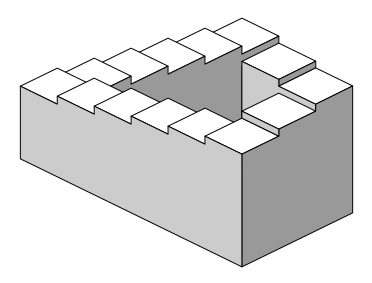
\includegraphics[width=.5\textwidth]{img/penrose}
	\caption{Verwirrung}
	\label{fig:penrose}
\end{figure}
\begin{thebibliography}{9}
\bibitem{dijkstra}
	Skiena, S., \textsc{Dijkstra’s algorithm}, S. 225--227,\\
  \emph{Implementing Discrete Mathematics: Combinatorics and Graph Theory with Mathematica, Reading, MA: Addison-Wesley},
  1990
\end{thebibliography}
\newpage
\subsection*{Minimale Pfade}
\label{app:paths}
Die Höhen der Felder sind in den folgenden Abbildungen als Heatmaps dargestellt, wobei hellere Farbtöne höhere Erhebungen darstellen.
\begin{center}
	\begin{minipage}[t]{.3\textwidth}
		\centering
		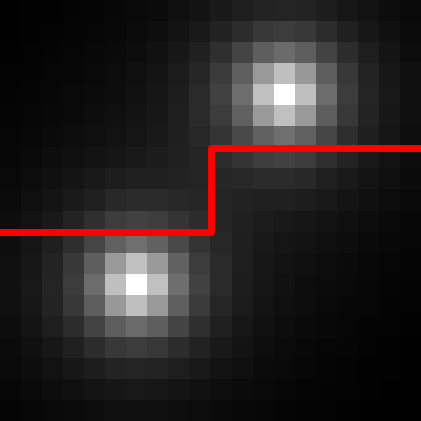
\includegraphics[width=\textwidth]{img/resized1}\par
		\ttfamily wildschwein1.txt
	\end{minipage}\hfill
	\begin{minipage}[t]{.3\textwidth}
		\centering
		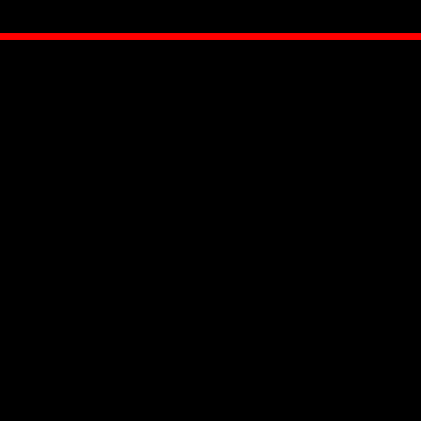
\includegraphics[width=\textwidth]{img/resized2}\par
		\ttfamily wildschwein2.txt
	\end{minipage}\hfill
	\begin{minipage}[t]{.3\textwidth}
		\centering
		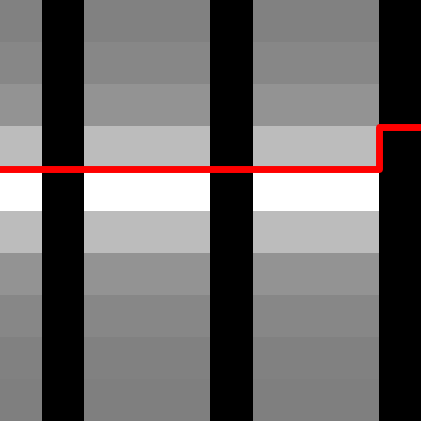
\includegraphics[width=\textwidth]{img/resized3}\par
		\ttfamily wildschwein3.txt
	\end{minipage}
	\vspace{1em}

	\begin{minipage}[t]{.3\textwidth}
		\centering
		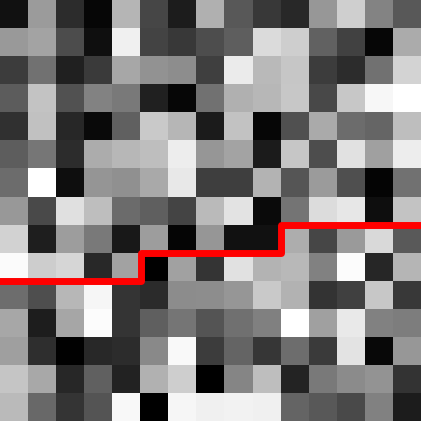
\includegraphics[width=\textwidth]{img/resized4}\par
		\ttfamily wildschwein4.txt
	\end{minipage}\hspace*{6mm}
	\begin{minipage}[t]{.3\textwidth}
		\centering
		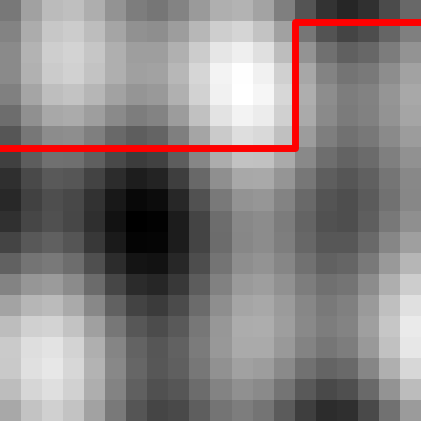
\includegraphics[width=\textwidth]{img/resized5}\par
		\ttfamily wildschwein5.txt
	\end{minipage}
\end{center}
\end{document}